\documentclass[11pt,twocolumn]{article}
\usepackage[T1]{fontenc}
\usepackage[utf8]{inputenc}
\usepackage{xcolor}
\definecolor{darkblue}{rgb}{0,0,0.5}
\usepackage[colorlinks=true,allcolors=darkblue]{hyperref}
\usepackage{amsmath}
\usepackage{amssymb}
\usepackage{booktabs}
\usepackage{enumitem}
\setlist{noitemsep}
\usepackage{caption}
\usepackage{subcaption}
\usepackage{graphicx}
\graphicspath{{image/}}
\usepackage[sorting=ynt,style=authoryear,uniquename=false]{biblatex}
\addbibresource{paper.bib}

\DeclareUnicodeCharacter{FFFD}{\unk}
\DeclareUnicodeCharacter{2588}{\eos}
\protected\def\unk{
\includegraphics[width=1ex]{unk.pdf}}
\protected\def\eos{
\includegraphics[width=1ex]{eos.pdf}}

\title{Glyph embedding for neural machine translation}
\author{%
  Kuan Yu\\
  \texttt{kuanyu@uni-potsdam.de}\\
  \\
  Master's Program in \emph{Cognitive Systems}\\
  University of Potsdam}
\date{February 2019}

\begin{document}
\maketitle

\begin{abstract}
  We explored the possibility of using glyph images as character embedding for neural machine translation
  with a simple recurrent attentional encoder-decoder architecture.
  We found that as the input to the decoder,
  glyph embedding worked as effectively as learned character embedding,
  even when the writing system was not logographic.
  We also tried glyph prediction and successfully performed end-to-end language translation on the written form.
  In this paper we analyzed the successes and failures of our models
  to summarize the advantages of our glyph-based approach
  in comparison to the conventional text-based approach,
  and proposed exciting possibilities for future works.
\end{abstract}

\section{Introduction}\label{sec:introduction}

Language stored in text format on computers rely on a standard of character encoding,
where each character is assigned a code point.
Sequences of characters, namely strings,
are generated from the set of characters through the free monoid construction,
also known as the Kleene closure in computer science.
This method of encoding has been the basis of natural language processing.
Expert systems model language at the symbolic level.
Symbols are strings representing words or phrases,
which are treated as discrete units and used for constructing larger units of language,
such as sentences, paragraphs, or whole texts.
The relations between symbols are stored externally as logical rules.
With the successful and wide adoption of statistical models,
especially deep neural networks,
symbols require an additional layer of encoding.
Statistical methods typically pick a minimal level of units to treat as discrete values.
Common choices for the modeling level are words, ngrams, or characters.
The starting point is then to embed the set of minimal units in a vector space as the standard basis.
This is known as one-hot encoding.
Often a linear transformation is applied to the one-hot vectors,
to model the linguistic relations between these units by their geometric relations.
This learned linear transformation is called a learned embedding.
Larger units are then composed from the vector representation of these minimal units through algebraic operations.
In this work, we adopt a nostalgic approach based on writing systems.
We use glyph images as character embedding in the task of neural machine translation (NMT).

NMT systems typically translate sentence strings from a source language
to sentence strings in a target language.
When a format other than text is required, such as speech,
it is common to compose the text translation system
with a speech recognition and/or synthesis system in a pipeline \parencite{speech-to-speech}.
End-to-end speech translation,
which usually refers to speech-to-text translation,
is an active field of research \parencite{berard2018end,vila2018end},
while research into direct speech-to-speech translation is uncommon \parencite{serdyuk2018towards}.
To our knowledge,
this is the first attempt at end-to-end written language translation.
On top of showing that translation directly on the written form is possible
and just as effective as text translation under certain conditions,
we demonstrate the advantages of our approach over the conventional text-based approach
with a careful examination of the successes and failures of our glyph-based models.

In this paper we first describe the background in NMT (Section~\ref{sec:background}),
then explain our experiments (Section~\ref{sec:experiments}),
and finally describe our results (Section~\ref{sec:results})
and present our conclusion (Section~\ref{sec:conclusion}).
An open-source implementation for our experiments is available in Python3 using Tensorflow.%
\footnote{\scriptsize{\url{https://github.com/lepidodendron/lepidodendron}}\\
  This project is a joint-effort of the author and Bailey Polonsky at the University of Potsdam.}

\section{Background}\label{sec:background}

\subsection{Neural machine translation}\label{sec:neur-mach-transl}

Recurrent neural network (RNN) with an encoder-decoder structure has led to the success of NMT systems
\parencite{kalchbrenner2013recurrent,sutskever2014sequence,cho2014learning,cho2014properties,wu2016google}.
The encoder RNN receives a sequence of vectors from the source language,
typically a sentence encoded on the word level,
and produces a single state vector which encodes the sentence.
The decoder autoregressively generates a sequence in the target language,
with each step conditioning on the encoded state and previously generated partial sequence.
The conditioning is conducted by the decoder recurrent state,
initialized from the encoded state.
Figure~\ref{fig:autoreg} shows the corresponding graphical model.

\begin{figure}
  \centering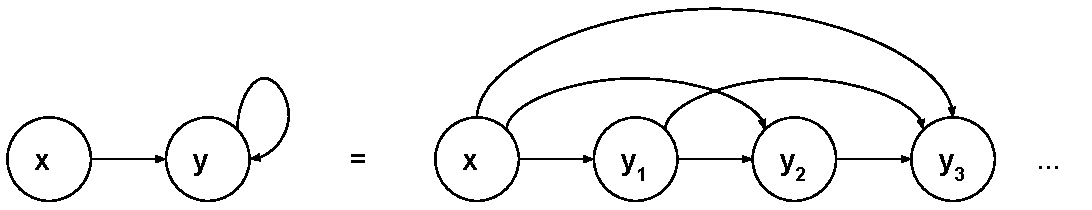
\includegraphics[width=\linewidth]{autoreg.pdf}
  \caption[]{\label{fig:autoreg}An autoregressive encoder-decoder models
    the probability of a target sequence \(y\) given a source sequence \(x\),
    with the target sequence factorized causally by position:
    \small{\( p(y \mid x) = p(y_{1} \mid x)\ p(y_{2} \mid y_{1}, x)\ p(y_{3} \mid y_{2}, y_{1}, x)\ \ldots \)}}
\end{figure}

During inference, an output is sampled from the decoder predictions at each step,
and fed back together with the recurrent state for the next step.
Since the search space grows exponentially for such a structure prediction problem,
beam search is commonly used to approximate the optimal solution \parencite{freitag2017beam}.
A cheaper alternative is greedy decoding,
where the sampling is simply performed by picking the prediction with the highest probability.
For training an autoregressive model,
the teacher-forcing method is typically used \parencite{williams1989learning}.
Instead of running the feedback loop,
the true target sequence is given as input with a begin-of-sentence (BOS) symbol padded at the front,
to predict the same sequence with an end-of-sentence (EOS) symbol padded at the end.

More recent works favor various attention mechanisms to counter
the drawback of having to encode a whole sequence into a single state vector
\parencite{bahdanau2014neural,luong2015effective}.
The encoder RNN produces an annotation vector for each position in the source sequence,
and for each decoding step,
the annotation vectors are summarized into a single context vector using attention
according to the recurrent state.
The context vector is then combined with the recurrent output in the decoder.
A particularly effective attention mechanism is multi-head scaled dot-product attention
used in the Transformer architecture \parencite{vaswani2017attention}.

\subsection{Modeling level}\label{sec:modeling-level}

While words are a common and intuitive choice for the basic units of sentences,
it has many drawbacks.
The vocabulary size is huge, often in an order of magnitude around or above \(10^{6}\),
resulting in a large number of parameters in the embedding matrix.
On top of that, due to their power law distribution,
the majority of words in the vocabulary of a language remains unseen in the available training data,
and most words in the observed vocabulary occur infrequently.
Furthermore, morphology is an important part of language,
especially for agglutinative languages,
which can only be modeled at the subword level.
Current approaches often augment word-level modeling with subword units \parencite{sennrich2015neural,kudo2018subword}.

Modeling at the character-level can be effective as well \parencite{kalchbrenner2016neural}.
However, characters also follow a power law or exponential distribution.
The Unicode encoding contains over \(10^{6}\) code points with \(137\,439\) defined so far,
the vast majority of which never occur in any single corpus.
At the same time, character crossover from another language is common.
Even on the character-level,
it is difficult if not impossible to model a language fully.

Moreover, languages with logographic writing systems encode certain semantic information below the character level.
Their compositional structures can only be retrieved from the character glyphs.
Learning an embedding from glyphs has shown to be valuable \parencite{su2017learning}.

\section{Experiments}\label{sec:experiments}

\subsection{Dataset and preprocessing}\label{sec:datas-prepr}

We used the European Parliament Proceedings Parallel Corpus
for German to English translation \parencite{koehn2005europarl}.
The reason for not choosing a logographic language is that we wish to verify
the general applicability of our approach.

We kept only parallel instances with sentences containing 3--256 characters.
The lower threshold was set to remove trivial instances,
and the upper threshold was set for the ease of experimentation.
We randomly picked 4\,096 instances for validation,
and used the remaining 1\,574\,071 instances for training.

We considered the subset of characters with 99.95\% coverage to be the frequent characters.
In the source language German, 78 out of 306 observed characters are frequent,
and in the target language English, 72 out of 293 are frequent.

\subsection{Glyph rendering}\label{sec:glyph-rendering}

For rendering the character glyphs,
we used the Pillow\footnote{\scriptsize{\url{https://python-pillow.org/}}} library
with the Noto Sans Mono\footnote{\scriptsize{\url{https://www.google.com/get/noto/}}} font.
Each glyph was rendered as an image with pixels in grayscale scaled in range \([0,1]\).

Individually rendered glyph images vary in size.
We fixed the height and width to the maximum value among the frequent characters.
With font size 20, the height for German and English glyphs was respectively 25 and 20 pixels.
The width was 12 pixels for both.
Each rendered image was flattened into a vector.
There vectors were the glyph embedding.

\begin{figure}
  \centering
  \begin{subfigure}[b]{0.5\linewidth}
    \centering
    
\includegraphics[width=0.3\linewidth]{glyph_src.pdf}
    \caption[]{German}
  \end{subfigure}%
  \begin{subfigure}[b]{0.5\linewidth}
    \centering
    
\includegraphics[width=0.3\linewidth]{glyph_tgt.pdf}
    \caption[]{English}
  \end{subfigure}
  \caption[]{\label{fig:glyph}Mean of glyphs.}
\end{figure}

We used the whitespace character as BOS paddings and the full block character █ as EOS paddings.
We also used the replacement character � for unknown characters,
which during training were the infrequent ones.
The treatment for unknown characters is only relevant in trials
where we used one-hot encoding instead of glyph embedding.
When glyphs are used, we always rendered the original character
with no special treatment for the rare ones.

Glyph rendering was a severe bottleneck for the training speed.
To solve this problem,
we cached the frequent glyphs,
and only rendered the rare ones on the fly.

\subsection{Experiment setup}\label{sec:experiment-setup}

We conducted four main trials,
varying the type of values connected to the model in three locations:
the encoder input, the decoder input, and the decoder output.
We use \texttt{g} to denote when a location is connected to glyphs,
and \texttt{c} when it is connected to one-hot encoded characters.

When one-hot encoding is used for the input,
the linear transformation in the first input layer acts as a learned embedding.
Therefore our trials was designed to compare the behaviors of learned embedding and glyph embedding.
The four trials were \texttt{ccc}, \texttt{cgc}, \texttt{cgg}, and \texttt{ggg}.
As an elaboration, in trial \texttt{cgc} the encoder used learned embedding
while the decoder used glyph embedding but predicted characters instead of glyphs.
Trial \texttt{ccc} was the baseline in line with conventional text-based translation.
Trial \texttt{ggg} performed end-to-end translation on the written form.

In order to compute the BLEU scores for evaluating the translation quality,
we needed the predictions in text format.
Whenever a model was trained to predict the glyphs,
we also included an additional output layer for predicting the characters.

\subsection{Model architecture}\label{sec:model-architecture}

For the encoder, we used 3 layers of stacked bidirectional RNN
with gated recurrent units (GRU) \parencite{cho2014learning}.
The decoder consisted of 3 layers of unidirectional GRU RNN,
followed by an 8-head scaled dot-product attention layer \parencite{vaswani2017attention}
with residual connection \parencite{he2016deep}
and layer normalization \parencite{ba2016layer}.
When a model was trained to predict characters,
we placed a fully-connected layer after attention to predict the logit probabilities over the character set,
which included the frequent characters, the proxy unknown character, and the proxy EOS character.
When a model was trained to predict glyphs,
we placed a fully-connected layer after attention with one unit for each pixel.
Figure~\ref{fig:arch} shows the architecture when both predictions were included.

\begin{figure}
  \centering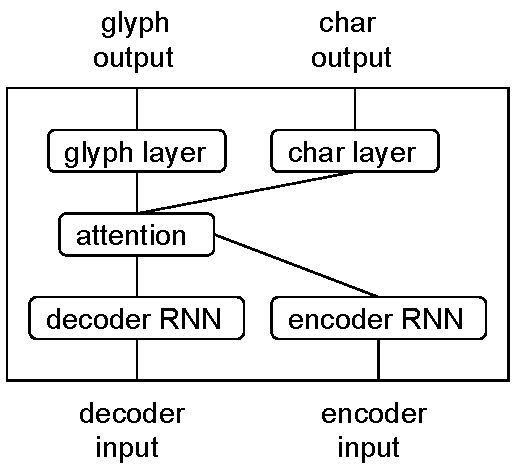
\includegraphics[width=0.8\linewidth]{image/architecture.pdf}
  \caption[]{\label{fig:arch}The architecture with both glyph and character predictions.}
\end{figure}

The loss function for character prediction was softmax cross-entropy (XENT).
For glyph prediction, we clipped the outputs in range \([0,1]\)
and computed the mean absolute error (MAE) for the loss.
Since the MAE loss was roughly \(1/10\) of the XENT loss,
when both losses were included,
we used \(10 \times \mathrm{MAE} + \mathrm{XENT}\) as the total weighted loss.
During training,
we monitored the accuracy of character prediction in teacher-forcing mode
as a criterion for fitting and overfitting.

We explored a few alternatives.
For the glyph prediction loss,
we tried sigmoid cross-entropy,
MAE with sigmoid activation,
MAE without clipping,
and mean squared error.
We also tried connecting the character layer after the glyph layer.
We found there alternatives less effective.

The models were trained with stochastic gradient descent using Adam optimization \parencite{kingma2014adam}.
The learning rate was scheduled \(lr / \left( 1 + dr \times \sqrt{s} \right))\) by the training step \(s\),
where \(lr = 0.001\) was the initial learning rate
and \(dr = 0.01\) was the decay rate.
We applied 10\% dropout \parencite{srivastava2014dropout} between the RNN layers
and after the attention layer right before the residual connection.

We trained the models with mini-batches of 128 instances.
Model \texttt{ccc} started to overfit after 30 epochs.
The other models except for \texttt{cgc} did not reach the optimal accuracy,
but we stopped training after 60 epochs.
Despite being underfit, \texttt{cgg} reached a higher validation accuracy than \texttt{ccc} and \texttt{cgc},
indicating a positive regularization effect when glyphs were used in the decoder.

\section{Results}\label{sec:results}

\subsection{Inference modes}\label{sec:inference-modes}

During autoregressive inference, the decoder prediction is fed back as the input for the next step.
Glyph prediction is a deterministic process,
while character prediction is probabilistic,
for which we used greedy decoding.
A model which was trained to predict both glyphs and characters
sometimes disagreed in the two types of predictions (see~\ref{sec:mism-betw-glyph}).
We discovered that it worked well to simply match the predicted glyph to the closest character
using MAE as a distance measure.
This can be seen as a method of discrete quantization:
One may consider converting the distance measures to probabilities,
making the glyph prediction process probabilistic.
We can likewise make character prediction deterministic,
by using the probability vector as feedback instead of sampling for a one-hot vector,
or by producing a fuzzy glyph averaged according to the predicted probabilities if glyphs are required as input.
In total we devised five modes of inference.

\begin{enumerate}
\item Use the predicted glyph as feedback and the predicted character for evaluation.
\item Use the predicted glyph as feedback and the closest matching character for evaluation.
\item Match the predicted glyph to the closest character for evaluation and feedback;
  When glyphs are required as input, render a fresh glyph for the character.
\item Use the predicted character for evaluation and feedback; Render when required.
\item Use the predicted character for evaluation and the probabilities as feedback; Render and average when required.
\end{enumerate}

The inference process terminated when the length of the output sequence reached 256.
The predicted sentence was trimmed at the first EOS character.

\subsection{Results and analysis}\label{sec:results-analysis}

We computed the BLEU scores on the validation data using SacreBLEU \parencite{post2018call}.%
\footnote{With the \texttt{intl} tokenizer (\texttt{sacrebleu -tok intl}).}
Table~\ref{tab:bleu} shows the results.
A more detailed analysis with examples can be found in Appendix~\ref{sec:examples}.

\begin{table}[htbp]
  \centering
  \begin{tabular}[tb]{cccccc}
    \toprule
    mode &1 &2 &3 &4 &5\\
    \midrule
    \texttt{ccc} &n/a  &n/a  &n/a  &30.9 &20.3\\
    \texttt{cgc} &n/a  &n/a  &n/a  &30.9 &22.4\\
    \texttt{cgg} &22.9 &23.5 &26.5 &30.9 &24.1\\
    \texttt{ggg} &21.9 &22.2 &25.3 &30.2 &23.0\\
    \bottomrule
  \end{tabular}
  \caption[]{\label{tab:bleu}BLEU scores.}
\end{table}

Mode 1 was the intended usage for the glyph-based models,
which suffered from the mismatch between the two types of predictions.
Mode 2 avoided this problem.
Mode 3 benefited from receiving freshly rendered glyphs as feedback
instead of relying on the predicted glyphs which were sometimes fuzzy.
Mode 4 conformed to the conventional greedy decoding method and produced the best results.
Mode 5 relied on the character prediction but intentionally made the input fuzzy
by using the probabilities instead of sampling from them.
The results from mode 5 shows that the conventional \texttt{ccc} model suffered
from the uncertainty introduced by forcing a probabilistic process to be deterministic,
whereas the glyph-based models were more robust (see~\ref{sec:robustn-against-fuzz}).

The two modes which treated translation as a probabilistic process (mode 3\&4)
produced better results than the deterministic modes.
This was due to the nature of the task.
During translation,
the model often faced multiple possibilities in structuring and wording (see~\ref{sec:decision-points}).
A probabilistic treatment allowed the model to trim the hypothesis space along the autoregressive process
and settled on one eventuality.
Since glyph prediction made the process deterministic,
the modes which relied on glyphs (mode 1\&2\&3) produces suboptimal results.
However, model \texttt{cgc} and \texttt{cgg} were as good as the conventional \texttt{ccc}
when the character prediction was consulted (mode 4).
One major advantage of using the glyph prediction was that even rare characters could be predicted,
and did not have to be treated as unknowns (see~\ref{sec:unkn-char}).

The fully glyph-based \texttt{ggg} performed worse than \texttt{cgg}.
The encoder was less effective when glyphs were used as the input.
The Latin script used for the source language provided no advantage to the encoder.

\subsection{Miscellaneous results}\label{sec:misc-results}

We conducted a follow-up experiment for Chinese to English translation
using the United Nations Parallel Corpus \parencite{ziemski2016united}.
We set the upper threshold for the sentence length to 128,
resulting in 7\,392\,227 training instances,
and tested with 4\,096 instances.
The Chinese glyphs were fixed to height 25 and width 20,
and 2\,681 out of 6\,357 character were frequent.
We trained \texttt{cgg} and \texttt{ggg} with mini-batches of size 256 for 12.8 epochs.
In mode 2, \texttt{ggg} performed slightly better than \texttt{cgg} (32.3 vs 31.6 BLEU).
However \texttt{cgg} performed better in a few other modes.
The effectiveness of the encoder when using glyphs for a logographic language was inconclusive.
The architecture of our models was not suitable for extracting subglyph structures
such as the composition of radicals.

We also experimented with the Transformer architecture \parencite{vaswani2017attention}
which used self-attention instead of recurrent layers.
Since the complexity of self-attention is quadratic with respect to the sequence length,
we had to restrict the model to only 2 layers and 256 hidden dimensions
in order to match the memory usage and training speed of our RNN models.
The reduced model was not able to learn glyph-based translation.

\section{Conclusion}\label{sec:conclusion}

In this work we explored the possibility of using glyph images as character embedding for machine translation
and successfully performed end-to-end language translation on the written form
with a simple recurrent attentional encoder-decoder architecture.

With probabilistic inference,
glyph embedding in the decoder works as effectively as learned embedding for characters,
even when the writing system is not logographic.
One major advantage with glyph embedding is that rare characters do not have to be treated as unknowns,
and the entire character set can be modeled fully.

With deterministic inference,
glyph-based models are more robust in the presence of fuzzy predictions
in comparison to conventional text-based models.
This is valuable when we wish to avoid the search space for fast translations.
Without treating each decoding step as a random variable,
the model is not truly autoregressive,
which is supported by the fact that fuzzy predictions could occur very early
without affecting the decisions regarding the structuring and the wording of the rest of the sentence
(see~\ref{sec:decision-points},~\ref{sec:fail-liter-transl},~\ref{sec:robustn-against-fuzz}).
Autoregressive models tend to behave well at the beginning and degenerate as mistakes accumulate.

The pseudo autoregressive behavior of our glyph-based models suggests that glyph embedding and glyph prediction
may yield more benefits in a non-autoregressive design \parencite{gu2017non},
using techniques such as denoising and iterative refinement \parencite{lee2018deterministic},
introducing latent variables \parencite{kaiser2018fast},
and probability density distillation \parencite{oord2017parallel}.

For future works along the glyph-based approach,
one may consider using a convolutional network
to learn the subglyph composition for a logographic language.
Transposed convolution may be used for non-autoregressive decoding.
Further more, each sentence may be treated simply as a continuous image,
without being segmented into monospaced glyphs.
This allows for efficient training using other font types and even handwritten data.
For producing the output in text format,
one may consider a postprocessing network for character or word predictions
with connectionist temporal classification \parencite{graves2006connectionist,libovicky2018end}.

\printbibliography[]

\appendix
\onecolumn

\section{Examples}\label{sec:examples}

Here we include some examples from the validation data.
Each example is an image of 3 or 4 lines.

\begin{enumerate}
\item The source sentence given as input to the model.
\item The target sentence for reference.
\item The glyph prediction from model \texttt{cgg}.
\item The glyph prediction from model \texttt{ggg} (optional).
\end{enumerate}

Each image is followed by the character predictions.
These examples demonstrate the behavior of our models in mode 1.
The sentence length is limited to 64 characters.

As a reminder, the full block character █ is used to signal EOS,
which appears as a white block in the images.
And the replacement character � stands for unknown characters,
which only occurs in the character predictions.
Many fuzzy glyphs resemble the mean of glyphs in Figure~\ref{fig:glyph}.

\subsection{Decision points}\label{sec:decision-points}

A comparison between the \texttt{cgg} and \texttt{ggg} predictions
revealed some choices the model had to face.
At those decision points, the glyphs were fuzzy.

\vspace{1.2em}\noindent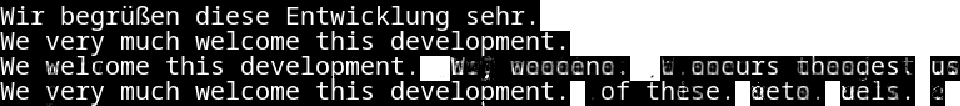
\includegraphics[width=\linewidth]{143.pdf}
\texttt{cgg}: \texttt{We velcome this development.█ SS  werkine.█ O wncurs toisgest█.s}\\
\texttt{ggg}: \texttt{We very much welcome this development.█ of these.█ eth █uels.█.█}\\

\vspace{-0.8em}
Model \texttt{cgg} was tempted to produce the ``v'' in very,
but simply produced ``welcome'' instead,
resulting in a fuzzy ``w'' in the glyph prediction and ``velcome'' in the character prediction.

\vspace{1.2em}\noindent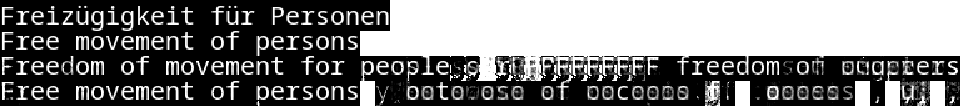
\includegraphics[width=\linewidth]{038.pdf}
\texttt{cgg}: \texttt{Free om of movement for people███████████████free om on migpeers}\\
\texttt{ggg}: \texttt{Free movement of persons█y brto ovc of tucomaa o.█.ortei █.██(█(}\\

\vspace{-0.8em}
``Freedom'' vs ``Free''; ``people'' vs ``persons''.

\vspace{1.2em}\noindent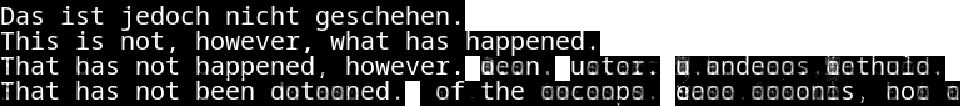
\includegraphics[width=\linewidth]{077.pdf}
\texttt{cgg}: \texttt{That has not happened. however.█Nesn.█ustir.█  andenl. Tuthuld.█}\\
\texttt{ggg}: \texttt{That has not heen drtammed.█.af the sucomda.█Aask Aitomis. hot i}\\

\vspace{-0.8em}
Model \texttt{ggg} mistook the structure for a passive voice construction,
and tried to produce a similar structure in English,
but failed to find a suitable verb.

\vspace{1.2em}\noindent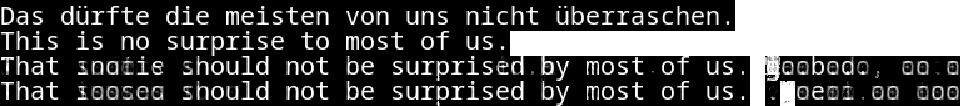
\includegraphics[width=\linewidth]{312.pdf}
\texttt{cgg}: \texttt{That itdris should not ce surprised.ay most.of us.█.asbod.  au t}\\
\texttt{ggg}: \texttt{That stvses should not be surprised by most of us.█.█.er  an tun}\\

\vspace{-0.8em}
Both model erroneously tried to translate with the passive voice,
and failed to find a suitable word to fill the subject position.
The failure occurred before the passive construction,
indicating that the decision was not made causally.

\subsection{Mismatch between glyph and character predictions}\label{sec:mism-betw-glyph}

\vspace{1.2em}\noindent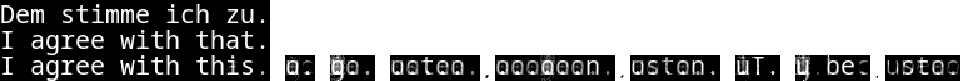
\includegraphics[width=\linewidth]{003.pdf}
\texttt{cgg}: \texttt{I agree.with thas.█..█.a.█.bt...█........█ust...█.T.█ .bel█.sta.}\\

\vspace{-0.8em}
Here the model struggled between ``this'' and ``that''.
The glyph prediction settled for ``this'',
even though it was unsure about the ``i'',
forcing the character prediction to become ``thas''.

\vspace{1.2em}\noindent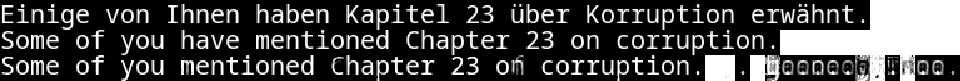
\includegraphics[width=\linewidth]{444.pdf}
\texttt{cgg}: \texttt{Some of you mentioned Chapter 23 of corruption.█ .█ as.e. █S█...}\\

\vspace{-0.8em}
``on'' vs ``of''.

\vspace{1.2em}\noindent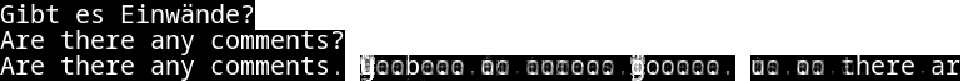
\includegraphics[width=\linewidth]{000.pdf}
\texttt{cgg}: \texttt{Are there any comments?█ a?be???an?ture?s??ook???█u???r there?ar}\\

\vspace{-0.8em}
Period vs question mark.

\vspace{1.2em}\noindent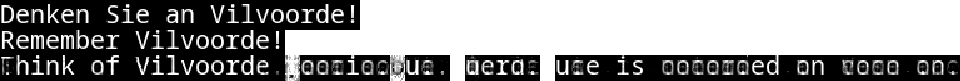
\includegraphics[width=\linewidth]{027.pdf}
\texttt{cgg}: \texttt{Think of Vilvoorde�R�aki��█u��█�ar��█use.is tuturaed�an aask��n�}\\

\vspace{-0.8em}
Period vs exclamation mark.

\subsection{Failure in literal translation}\label{sec:fail-liter-transl}

When the model tried to produce a literal translation following the structure of the source sentence,
it might fail to find a suitable word in the target language.

\vspace{1.2em}\noindent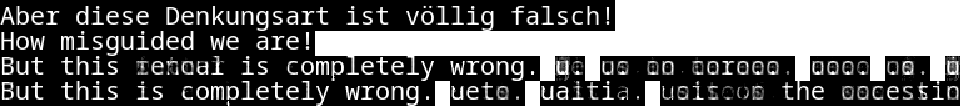
\includegraphics[width=\linewidth]{193.pdf}
\texttt{cgg}: \texttt{But this manoul is completely wrong.█��█����n aurr���█����█���█�}\\
\texttt{ggg}: \texttt{But this ms completely wrong�█ueti�█uasti��█usts  p the fttestin}\\

\vspace{-0.8em}
The word ``Denkungsart'' is difficult to translate.
Model \texttt{cgg} failed to find the translation,
while \texttt{ggg} avoided it altogether.

\vspace{1.2em}\noindent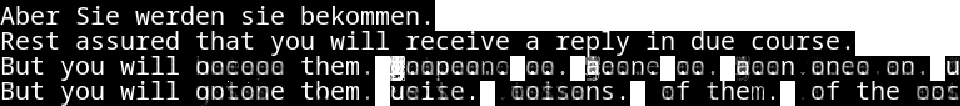
\includegraphics[width=\linewidth]{057.pdf}
\texttt{cgg}: \texttt{But you will brcopp them.█...n....█...█.esn.█...█.asn Cner.yu.█.}\\
\texttt{ggg}: \texttt{But you will gnli e them.█uetle.█.tunlens.█ if them.█.tf the Uuc}\\

\vspace{-0.8em}
Failed to translate ``bekommen''.

\vspace{1.2em}\noindent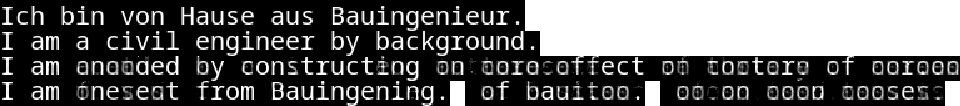
\includegraphics[width=\linewidth]{123.pdf}
\texttt{cgg}: \texttt{I am antuied by bonstructing futbarewfffect fn toutiri.bf bur.et}\\
\texttt{ggg}: \texttt{I am fnerert from Bauingening.█ af Bark..n.█.an tn tans.tensess█}\\

\vspace{-0.8em}
Failed to understand ``von Haus aus'' and translate ``Bauingenieur''.

% \subsection{Failure due to synonym confusion}\label{sec:fail-synonym-conf}

% \vspace{1.2em}\noindent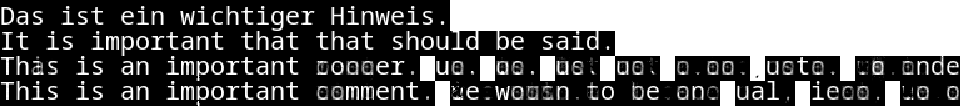
\includegraphics[width=\linewidth]{069.pdf}
% \texttt{cgg}: \texttt{This is an important polter.█unt█.a.█.at█urt█uamr █usti █B2 rnde}\\
% \texttt{ggg}: \texttt{This is an important plmment.█.eswiudh.to te ane█uali█ient.█utnm}\\

% \vspace{-0.8em}
% For translating ``Hinweis'',
% \texttt{ggg} produced the glyphs for ``comment'',
% but the character prediction might be ``point'',
% and \texttt{cgg} could not decider.

% \vspace{1.2em}\noindent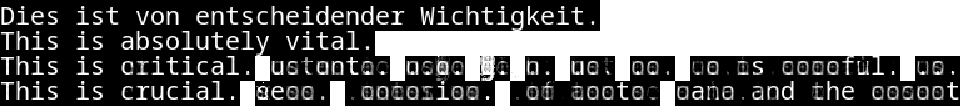
\includegraphics[width=\linewidth]{181.pdf}
% \texttt{cgg}: \texttt{This is vriticall█ stunt..█.. .█..█..█uet█.e.█ua is auveful.█.s.}\\
% \texttt{ggg}: \texttt{This is crucial.█ieds.█ wutkrios.█ if tuttoe█.ann.and ihe Eutult}\\

% \vspace{-0.8em}
% they found different words "critical" and "crucial"; the chars in cgg seem to be going for "vital"

% \vspace{1.2em}\noindent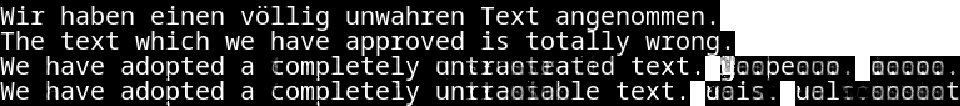
\includegraphics[width=\linewidth]{306.pdf}
% \texttt{cgg}: \texttt{We have adopted a tompletely untrubteated text.█ aspea...█.a....}\\
% \texttt{ggg}: \texttt{We have adopted a completely untransable text.█uats █uslt uptu t}\\

% \vspace{-0.8em}
% both failed to translated "unwahren"; cgg char tried to go for "totally" instead of "completely"

% \vspace{1.2em}\noindent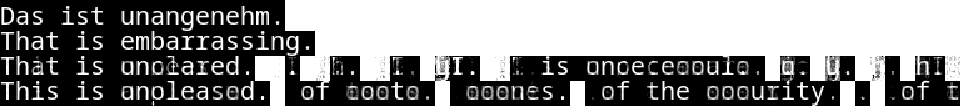
\includegraphics[width=\linewidth]{007.pdf}
% \texttt{cgg}: \texttt{That is unclased.█..██..██..█uTE██H is uncecembul..█.a█..██.█ T█}\\
% \texttt{ggg}: \texttt{This is anpleasid.█ if tonts.█.titkes.█.if the Etturity.█.█.if t}\\

% \vspace{-0.8em}
% For translating ``unangenehm'', both models seemed to be aiming for ``unpleasant'' but failed

\subsection{Failure in termination}\label{sec:failure-termination}

The glyph predictions were conservative about terminating the sentence.
Often when the predicted character was a period,
the predicted glyph was faint,
and the model produced unintelligible content after the point where it should have terminated.

\vspace{1.2em}\noindent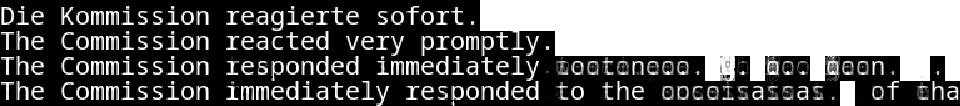
\includegraphics[width=\linewidth]{095.pdf}
\texttt{cgg}: \texttt{The Commission reaponded immediately.wint ne...██.█...█.ezn.██.█}\\
\texttt{ggg}: \texttt{The Commission rmmediately responded to the nttenvattat.█.if tha}\\

\vspace{1.2em}\noindent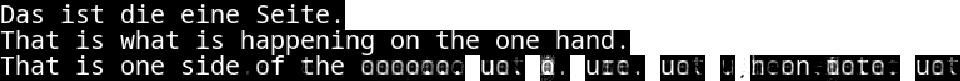
\includegraphics[width=\linewidth]{020.pdf}
\texttt{cgg}: \texttt{That is one side.of the ppc....█.s.█..█urt.█urt█.█rianesrth █ust}\\

\vspace{-0.8em}
Could have stopped at ``one side''.

\vspace{1.2em}\noindent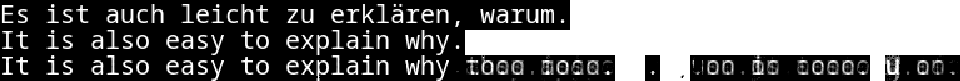
\includegraphics[width=\linewidth]{157.pdf}
\texttt{cgg}: \texttt{It is also easy to explain why.toou.iusk.██.██ in in turt █u an}\\

\vspace{-0.8em}
Could have stopped at ``why''.

\vspace{1.2em}\noindent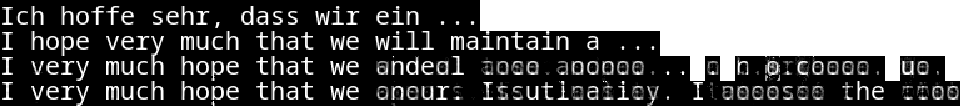
\includegraphics[width=\linewidth]{098.pdf}
\texttt{cgg}: \texttt{I very much hope that we wnderl ..t  .n u ....█.█....chrk. █ e █}\\
\texttt{ggg}: \texttt{I very much hope that we .neur..�f.u....li....I .lsosee..he....s}\\

\vspace{-0.8em}
Both models could not decide how to terminate the sentence due to its incompleteness.

\subsection{Hour format}\label{sec:hour-format}

\vspace{1.2em}\noindent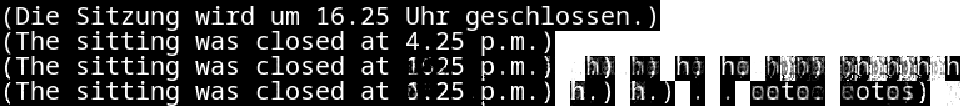
\includegraphics[width=\linewidth]{235.pdf}
\texttt{cgg}: \texttt{(The sitting was closed at 4.25 p.m.)██.)█..█h.█h.█D█C.█ChCCChCh}\\
\texttt{ggg}: \texttt{(The sitting was closed at 4.25 p.m.)█h.)█h.)█.█.█.ete-█.otes)██}\\

\vspace{-0.8em}
Failure.

\vspace{1.2em}\noindent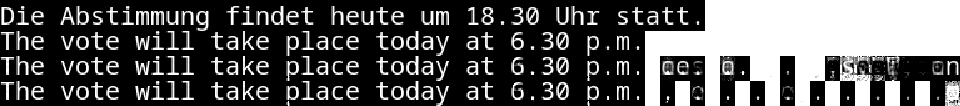
\includegraphics[width=\linewidth]{287.pdf}
\texttt{cgg}: \texttt{The vote will take place today at 6.30 p.m.█.a.█..██.██  █ CRwtn}\\
\texttt{ggg}: \texttt{The vote will take place today at 6.30 p.m.█.█.█.█.█.█.█.█.█.█.(}\\

\vspace{-0.8em}
Success.

\subsection{Unknown characters}\label{sec:unkn-char}

Rare characters could be predicted with the correct glyphs,
whereas the character prediction could only produce � since they were treated as unknowns during training.

\vspace{1.2em}\noindent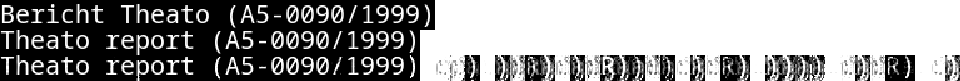
\includegraphics[width=\linewidth]{058.pdf}
\texttt{cgg}: \texttt{Theato report (A5-0090�1999)███S█ █  █ █ E █ █ █  █ S█ ██ █ )██}\\

\vspace{1.2em}\noindent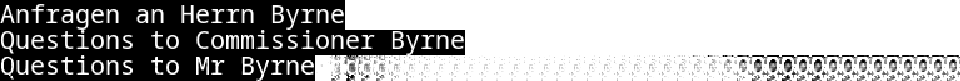
\includegraphics[width=\linewidth]{019.pdf}
\texttt{cgg}: \texttt{�uestions to Cr Byrne███████████████████████████████████████████}\\

\vspace{1.2em}\noindent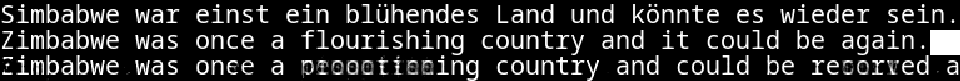
\includegraphics[width=\linewidth]{517.pdf}
\texttt{cgg}: \texttt{�imbabwe was once a pron ri ging country and could be reptrved.a}\\

\subsection{Robustness against fuzzy predictions}\label{sec:robustn-against-fuzz}

When the model predicted fuzzy glyphs for some words,
the rest of the sentence could still follow through,
even though the model had never seen a fuzzy glyph during training.

\vspace{1.2em}\noindent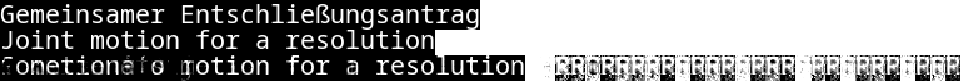
\includegraphics[width=\linewidth]{097.pdf}
\texttt{cgg}: \texttt{Joneriona   motion for a resolution█████████J███████████████████}\\

\vspace{1.2em}\noindent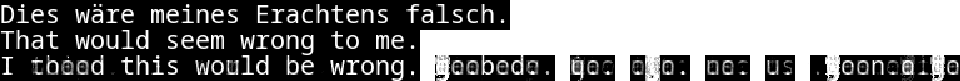
\includegraphics[width=\linewidth]{116.pdf}
\texttt{cgg}: \texttt{I tolr  this would be wrong.█ asbed..█ e.█  ..█Nat█ s█ (ooniuldr}\\

\vspace{1.2em}\noindent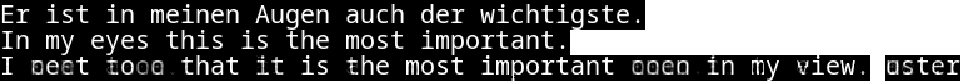
\includegraphics[width=\linewidth]{223.pdf}
\texttt{cgg}: \texttt{I tett to k that it is the most important.oucn.in my view.█uster}\\

\end{document}
